\chapter{Ondas, modos cuantizados y operadores de creación}

\section{Ondas, campos y exponenciales complejas}

La teoría cuántica de campos es la herramienta básica de la física de partículas. Antes de ofrecer siquiera una explicación elemental de un campo cuántico, conviene reunir los hechos matemáticos que relacionan las ondas con las partículas. Una onda ya es una configuración de campo: un campo varía de un punto a otro del espacio, y una onda es una configuración en la que esos valores oscilan y se propagan. La mecánica cuántica establece el vínculo entre estas ondas y las partículas.

Aquí se da por supuesto que el lector conoce la mecánica cuántica y la relatividad especial. El propósito inmediato es repasar los elementos necesarios para la física de partículas, no sustituir un curso de ninguna de esas materias.

Una exponencial se caracteriza por un crecimiento proporcional. Si
\begin{equation}
f(x)=e^{\alpha x},
\end{equation}
entonces
\begin{equation}
\frac{df}{dx}=\alpha f.
\end{equation}
En un intervalo pequeño, el incremento es proporcional a la cantidad que ya hay. El crecimiento de una población en una placa de Petri ofrece la imagen conocida: cuantos más organismos hay, más pueden reproducirse, de modo que la tasa de aumento es proporcional a la propia población. Multiplicar \(e^{\alpha x}\) por una constante global no altera esta propiedad definitoria.

El seno y el coseno oscilan en lugar de crecer. Son la misma curva desplazada un cuarto de ciclo, y al derivarlas se transforman la una en la otra:
\begin{align}
\frac{d}{dx}\sin(kx)&=k\cos(kx),\\
\frac{d}{dx}\cos(kx)&=-k\sin(kx).
\end{align}
Ninguna de las dos funciones por sí sola es una exponencial, porque su derivada es proporcional a la otra función. La combinación compleja sí tiene la propiedad exponencial. Dado que \(i^2=-1\),
\begin{align}
\frac{d}{dx}\bigl(\cos(kx)+i\sin(kx)\bigr)
&=-k\sin(kx)+ik\cos(kx)\\
&=ik\bigl(\cos(kx)+i\sin(kx)\bigr).
\end{align}
por tanto,
\begin{equation}
e^{ikx}=\cos(kx)+i\sin(kx).
\end{equation}
Esta identidad aparece una y otra vez porque los senos y cosenos describen oscilaciones ondulatorias. Cuando \(x\) es una coordenada espacial, la función oscila a través del espacio. Si el argumento es el tiempo, oscila en el tiempo.

\section{Frecuencia, longitud de onda y momento del fotón}

La frecuencia ordinaria \(f\) es el número de ciclos completos por segundo. Un ciclo es una oscilación completa. La frecuencia angular mide el mismo movimiento en radianes por segundo:
\begin{equation}
\omega=2\pi f.
\end{equation}
Ambas notaciones describen la misma frecuencia. Se pasa de una a otra para evitar factores innecesarios de \(2\pi\) en un cálculo, aunque esos factores nunca desaparecen del todo.

La longitud de onda \(\lambda\) es la distancia que ocupa un ciclo espacial completo. Si una onda se propaga con rapidez \(v\), el producto de la distancia por ciclo y el número de ciclos por segundo es la rapidez de propagación:
\begin{equation}
\lambda f=v.
\end{equation}
Para la luz en el vacío, \(v=c\), así que
\begin{equation}
\lambda f=c.
\end{equation}
Para una onda sonora, el miembro derecho es la rapidez del sonido; para una onda de agua, es la rapidez correspondiente a esa onda. Por tanto, la aparición de \(c\) es una afirmación sobre la luz, no una definición válida para todas las ondas.

La mecánica cuántica introduce la constante de Planck en dos notaciones,
\begin{equation}
\hbar=\frac{h}{2\pi}.
\end{equation}
Pasar de \(h\) a \(\hbar\) solo traslada factores de \(2\pi\) de una ecuación a otra.

Los valores numéricos de las constantes dimensionales dependen de las unidades empleadas para expresarlas. Los metros, segundos y kilogramos son convenciones a escala humana, prácticas para las longitudes y los tiempos ordinarios. Las unidades tradicionales comparables con la longitud de un brazo eran útiles para medir tela o cuerda; sea cual sea la trayectoria histórica precisa que condujo al metro, ningún principio fundamental selecciona esta escala humana particular. En unidades del SI,
\begin{equation}
\begin{aligned}
h &\simeq 6.6\times10^{-34}\ \mathrm{J\,s},
&\hbar &\simeq 1.1\times10^{-34}\ \mathrm{J\,s},\\
c &\simeq 3\times10^8\ \mathrm{m\,s^{-1}}.
\end{aligned}
\end{equation}
Lo que importa de estas cifras es su escala en unidades convencionales: la constante de Planck es extraordinariamente pequeña y la rapidez de la luz es extraordinariamente grande.

Un cuanto de un modo tiene energía
\begin{equation}
E_{\text{one quantum}}=\hbar\omega=hf.
\end{equation}
Esta es la energía de un fotón, no la energía total de una onda electromagnética clásica arbitraria. La luz visible tiene una frecuencia del orden de \(10^{15}\) ciclos por segundo, por lo que un fotón óptico típico tiene una energía del orden de
\begin{equation}
E_\gamma\sim 10^{-19}\ \mathrm{J}.
\end{equation}
Incluso una oscilación óptica tan rápida corresponde a una energía muy pequeña por cuanto, porque \(h\) es muy pequeña. Por eso, una cantidad macroscópica de energía óptica contiene un número enorme de fotones.

Conviene prestar especial atención a la energía y al momento, porque ambos se conservan. Son cantidades útiles para llevar la cuenta: la energía y el momento totales que entran en un proceso deben compensarse con la energía y el momento totales que salen de él. El momento es un vector y apunta en la dirección del movimiento. Para una partícula que se mueve mucho más despacio que la luz,
\begin{equation}
\vec p=m\vec v.
\end{equation}

Consideremos ahora radiación electromagnética colimada en una dirección, en vez de dispersa en muchas direcciones. Su momento apunta en la dirección del haz. La fórmula no relativista no se puede aplicar a un fotón, porque \(m\) representa la masa en reposo y el fotón tiene masa en reposo nula. Sin embargo, existe una regla mnemotécnica dimensional útil. Si se asigna \emph{de manera impropia} al fotón la cantidad \(E/c^2\) como si fuera una masa y luego se sustituye \(v=c\), se obtiene
\begin{equation}
mv\longrightarrow \frac{E}{c^2}c=\frac{E}{c}.
\end{equation}
Este procedimiento da casualmente el resultado correcto y también las unidades correctas, pero no es un argumento legítimo para afirmar que el fotón tiene masa en reposo \(E/c^2\). La afirmación relativista válida para la radiación colimada es
\begin{equation}
|\vec p|=\frac{E}{c}.
\end{equation}
La ecuación da el módulo. La dirección es aquella en la que se propaga la radiación.

Para un fotón,
\begin{align}
|\vec p_\gamma|
&=\frac{E_\gamma}{c}
=\frac{hf}{c}.
\end{align}
Para la luz,
\begin{equation}
\lambda f=c,
\qquad
\frac{f}{c}=\frac{1}{\lambda},
\end{equation}
y, por tanto,
\begin{equation}
|\vec p_\gamma|=\frac{hf}{c}=\frac{h}{\lambda}.
\end{equation}

\begin{figure}[t]
\centering
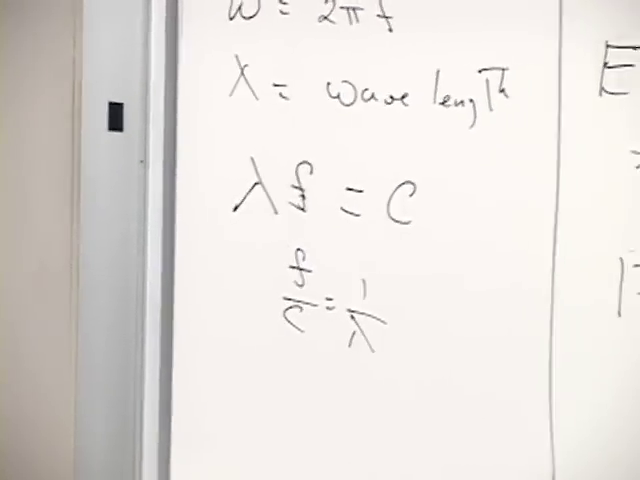
\includegraphics[width=0.56\textwidth]{lecture_02_figure_02.png}
\caption{Para la luz, \(\lambda f=c\) y \(f/c=1/\lambda\), relaciones que permiten obtener \(|\vec p_\gamma|=h/\lambda\).}
\lectureframe{00:21:39}
\end{figure}

Cuanto menor es la longitud de onda, mayor es el momento del fotón. Este es uno de los hechos cuánticos más importantes para la física de partículas. Para estudiar un objeto pequeño se necesita una sonda de longitud de onda corta, y esa longitud de onda corta tiene como contrapartida un momento grande.

\begin{classroomqa}
\lecturetimestamp{00:22:23}
\audiencequestion{¿Es \(E=\hbar\omega\) fundamental o se deduce de un principio más profundo?}
\lecturerresponse{Se deduce de la mecánica cuántica del oscilador armónico. Aquí usaremos ese resultado sin repetir su demostración; el formalismo del oscilador que desarrollaremos a continuación proporciona el contexto más profundo.}
\end{classroomqa}


\section{Amplitud de onda y número de fotones}

\begin{classroomqa}
\lecturetimestamp{00:23:10}
\audiencequestion{¿Qué significa la amplitud de una onda en términos de fotones?}
\lecturerresponse{Comparemos dos ondas con la misma longitud de onda y frecuencia, pero con amplitudes distintas, como \(\sin(kx)\) y \(A\sin(kx)\). Clásicamente, la energía en una región fija es proporcional al cuadrado de la amplitud. Cuánticamente, un modo que contiene \(n\) fotones tiene energía \(n\hbar\omega\). Por tanto, a frecuencia, región y normalización fijas, la amplitud crece, en orden de magnitud, como \(\sqrt n\).}
\end{classroomqa}

Las dos ondas tienen el mismo patrón de oscilación. Una es simplemente más intensa que la otra.\footnote{El esquema sigue la comparación de ondas de 00:23:47--00:24:28.}

\begin{figure}[t]
\centering
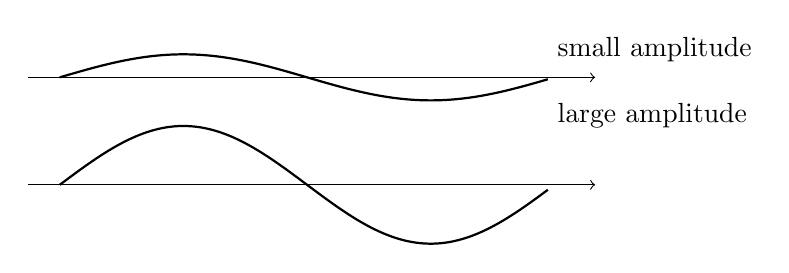
\begin{tikzpicture}[x=1cm,y=0.65cm]
\draw[->] (-0.4,0) -- (6.8,0);
\draw[->] (-0.4,-2.1) -- (6.8,-2.1);
\draw[thick] plot[domain=0:6.2,samples=120] (\x,{0.45*sin(\x r)});
\draw[thick] plot[domain=0:6.2,samples=120] (\x,{-2.1+1.15*sin(\x r)});
\draw (6.2,0.55) node[right]{small amplitude};
\draw (6.2,-0.75) node[right]{large amplitude};
\end{tikzpicture}
\caption{Ondas con igual longitud de onda y frecuencia, pero con amplitudes distintas.}
\end{figure}

Para una cantidad fija de onda,
\begin{equation}
E_{\text{wave}}\propto A^2.
\end{equation}
En el caso de una onda electromagnética, esto expresa el hecho conocido de que la energía del campo es proporcional al cuadrado de la intensidad del campo. Si el mismo modo contiene \(n\) fotones, entonces
\begin{equation}
E_{\text{wave}}=n\hbar\omega.
\end{equation}
En consecuencia, si se mantienen fijos el modo, la frecuencia, la normalización y la región,
\begin{equation}
A^2\propto n\hbar\omega,
\qquad
A\propto\sqrt n\quad\text{at fixed }\omega.
\end{equation}
No se afirma ninguna normalización exacta. Importa la cantidad de onda que se incluya: duplicar la longitud de una onda que, por lo demás, es uniforme cambia su energía total, pero no la amplitud local. Por tanto, la proporcionalidad puede entenderse para una región fija, como una longitud de onda.

También hay una salvedad específicamente cuántica. No se pueden asignar valores clásicos exactos a la amplitud y a la fase a la vez. Por eso, la pregunta ``¿Cuál es la amplitud de un fotón?'' es ambigua si pide un campo clásico perfectamente definido. Aun así, tomar \(n=1\) da una escala razonable de orden de magnitud.

\begin{classroomqa}
\lecturetimestamp{00:28:25}
\audiencequestion{¿Representa el desplazamiento vertical en un dibujo de una onda electromagnética la posición espacial del fotón?}
\lecturerresponse{No. El eje de propagación es espacial, mientras que la coordenada vertical representa el valor del campo eléctrico o magnético. El momento apunta a lo largo del eje de propagación, no en la dirección de la amplitud del campo representada en la gráfica.}
\end{classroomqa}

La onda puede propagarse en cualquier dirección espacial, pero el dibujo sinusoidal habitual usa solo el eje horizontal como coordenada espacial. La otra dirección representada indica la intensidad del campo.

\begin{classroomqa}
\lecturetimestamp{00:29:37}
\audiencequestion{¿Se cuenta el número de fotones indicado dentro de una longitud de onda o de un período de la onda?}
\lecturerresponse{Se puede elegir una región fija, como una longitud de onda. Por eso la relación es solo una proporcionalidad: la energía total y el número de fotones también dependen de cuánta onda se incluya. A la misma amplitud, dos, tres o cuatro longitudes de onda contienen, respectivamente, más energía que una.}
\end{classroomqa}

\begin{classroomqa}
\lecturetimestamp{00:30:17}
\audiencequestion{¿Carece de sentido hablar de la amplitud de un solo fotón?}
\lecturerresponse{Solo tiene sentido como afirmación de orden de magnitud, obtenida al tomar \(n=1\). En un modo electromagnético, la información sobre los campos eléctrico y magnético desempeña un papel análogo al de la información sobre la posición y el momento conjugados; por tanto, la incertidumbre cuántica limita la precisión con la que se puede asignar una amplitud clásica. La relación de orden de magnitud sigue siendo útil.}
\end{classroomqa}

Estas preguntas ya nos conducen a la teoría cuántica de campos, donde se puede formular con precisión la relación entre las variables de campo y el número de partículas. Por ahora bastan las proporcionalidades.

\section{Relaciones cuánticas generales y ondas de materia lentas}

Algunas de las fórmulas introducidas para los fotones se aplican de forma mucho más general; otras, no. Conviene distinguirlas antes de pasar a los electrones.

\begin{figure}[t]
\centering
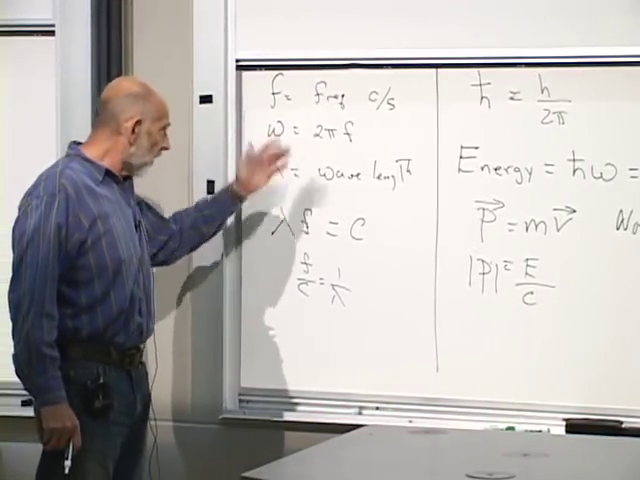
\includegraphics[width=0.82\textwidth]{lecture_02_figure_03.png}
\caption{Definiciones de onda y relaciones del fotón y del momento no relativista, comparadas según sus dominios de validez.}
\lectureframe{00:31:52}
\end{figure}

Las definiciones de \(f\), \(\omega=2\pi f\) y \(\lambda\) se aplican en general. La relación cuántica
\begin{equation}
E=\hbar\omega=hf
\end{equation}
también es general en la discusión que nos ocupa. En cambio, las fórmulas que contienen \(c\), como \(\lambda f=c\) y \(|\vec p|=E/c\), se aplican a ondas que se mueven a la velocidad de la luz. La fórmula \(\vec p=m\vec v\) se aplica a partículas que se mueven mucho más despacio que la luz. El movimiento relativista entre esos dos límites requiere una interpolación que todavía no necesitamos.

La relación entre el momento--y la longitud de onda se mantiene en el ejemplo del fotón:
\begin{equation}
p=\frac{h}{\lambda}.
\end{equation}
Aquí \(p\) denota el módulo cuando \(\lambda\) se toma como una longitud de onda positiva; la dirección puede especificarse por separado.

\begin{figure}[t]
\centering
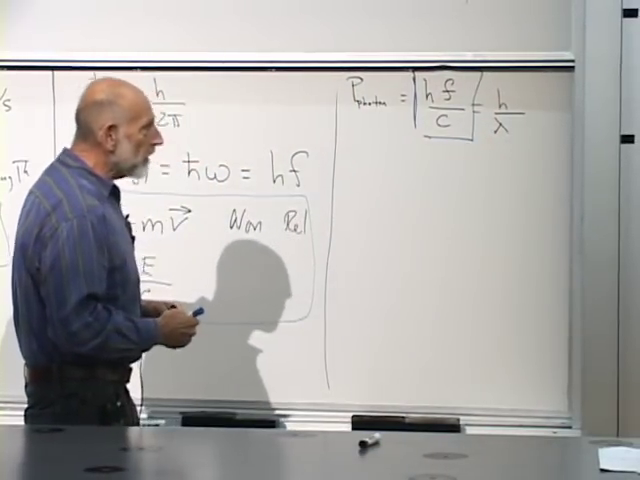
\includegraphics[width=0.74\textwidth]{lecture_02_figure_04.png}
\caption{Momento del fotón \(|\vec p_\gamma|=hf/c=h/\lambda\), que conduce a la relación general de de Broglie.}
\lectureframe{00:33:32}
\end{figure}

Se puede asociar una onda a un electrón, a un núcleo e incluso a una bola de bolos. La interferencia de electrones es una manifestación de este hecho. Escribamos la onda electrónica como \(\psi\). ¿Qué sustituye a \(\lambda f=c\) para un electrón que se mueve despacio? Falta incorporar la relación no relativista entre energía y momento.

Partamos de la energía cinética y del momento:
\begin{align}
E&=\frac12 mv^2,\\
p&=mv,
\qquad
v=\frac{p}{m}.
\end{align}
Al sustituir la última relación en la primera se obtiene
\begin{align}
E
&=\frac12m\left(\frac{p}{m}\right)^2\\
&=\frac{p^2}{2m}.
\end{align}
La masa aparece en el numerador de \(\frac12 mv^2\) y en el denominador de \(p^2/(2m)\). Es fácil confundir esa posición, así que conviene volver a deducirla.

Ahora usemos las relaciones cuánticas generales
\begin{equation}
E=hf,
\qquad
p=\frac{h}{\lambda}.
\end{equation}
Para una partícula lenta,
\begin{align}
hf
&=\frac{p^2}{2m}\\
&=\frac{1}{2m}\left(\frac{h}{\lambda}\right)^2\\
&=\frac{h^2}{2m\lambda^2}.
\end{align}
Al dividir por \(h\) se obtiene
\begin{equation}
f=\frac{h}{2m\lambda^2}.
\end{equation}

\begin{figure}[t]
\centering
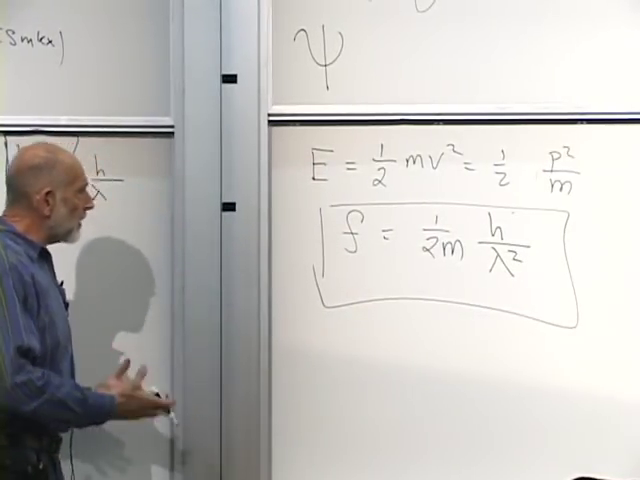
\includegraphics[width=0.64\textwidth]{lecture_02_figure_05.png}
\caption{Para una partícula lenta, \(E=p^2/(2m)\) y \(p=h/\lambda\) conducen a \(f=h/(2m\lambda^2)\).}
\lectureframe{00:37:47}
\end{figure}

Para la luz,
\begin{equation}
f\propto\frac{1}{\lambda},
\end{equation}
mientras que para la materia lenta,
\begin{equation}
f\propto\frac{1}{\lambda^2}.
\end{equation}
No hace falta memorizar la segunda relación por separado. Siempre se puede reconstruir a partir de \(E=p^2/(2m)\), \(E=hf\) y \(p=h/\lambda\). Para un electrón que se mueve lentamente en un átomo, da la frecuencia de la onda de Schr\"odinger correspondiente.

\begin{classroomqa}
\lecturetimestamp{00:38:35}
\audiencequestion{¿Se aplica a partículas distintas de los electrones la relación no relativista entre frecuencia--longitud de onda?}
\lecturerresponse{Sí. Se aplica a cualquier partícula que se mueva mucho más despacio que la luz. La interpolación relativista entre los límites de bajas velocidades y de movimiento a la velocidad de la luz es un tema aparte.}
\end{classroomqa}

\begin{classroomqa}
\lecturetimestamp{00:38:55}
\audiencequestion{¿Qué relación se aplica a un neutrino?}
\lecturerresponse{Depende de la velocidad del neutrino. La mayoría de los neutrinos que encontramos en la naturaleza se mueven muy cerca de la velocidad de la luz, por lo que la relación correspondiente al límite de la luz es una buena aproximación. En cambio, un neutrino que se moviera mucho más despacio que la luz obedecería la relación no relativista.}
\end{classroomqa}

\editorialnote{Un breve intercambio con el público, justo después de la pregunta sobre los neutrinos, trata sobre amplitudes, cuantos y distintas longitudes de onda de los electrones, pero el texto está demasiado dañado para reconstruirlo con seguridad. La respuesta que sí puede recuperarse aplaza la relación general entre amplitudes y cuantos con distintas longitudes de onda.}

\begin{classroomqa}
\lecturetimestamp{00:39:56}
\audiencequestion{¿Es lento o relativista un electrón de un acelerador de \(20\,\mathrm{keV}\)?}
\lecturerresponse{Se trata como lento. En unidades en las que \(c=1\), la masa, la energía y el momento pueden expresarse en las mismas unidades. La escala de la energía en reposo del electrón es aproximadamente \(0.5\,\mathrm{MeV}\), mientras que \(20\,\mathrm{keV}\) es mucho menor. Equivalentemente, el criterio no relativista para el momento es \(p\ll mc\).}
\end{classroomqa}

La comparación de energías en el ejemplo es
\begin{equation}
K=20\,\mathrm{keV}\ll m_ec^2\simeq0.5\,\mathrm{MeV}.
\end{equation}
\editorialnote{El pasaje original en 00:39:56--00:41:40 presenta \(20\,\mathrm{keV}\) como una energía del acelerador y luego formula el criterio relativista mediante la comparación de la cantidad de movimiento con la masa en reposo. Expresar por separado los criterios de energía cinética y de cantidad de movimiento evita equiparar la energía citada con una cantidad de movimiento y conserva la conclusión no relativista indicada.}

\section{Velocidad de fase, velocidad de grupo y dispersión}

\begin{classroomqa}
\lecturetimestamp{00:41:46}
\audiencequestion{¿Se puede obtener la velocidad de una onda electrónica multiplicando la frecuencia por la longitud de onda?}
\lecturerresponse{Ese producto da la velocidad de fase, no la velocidad atribuida al electrón. Un paquete localizado tiene una velocidad de fase, que describe el movimiento de sus crestas y valles internos, y una velocidad de grupo, que describe el movimiento de la envolvente. La velocidad de grupo se identifica con el movimiento de la partícula.}
\end{classroomqa}

Un paquete de ondas se parece localmente a una función seno o coseno, pero está confinado por una envolvente. Al desplazarse, la envolvente y las crestas que contiene no tienen por qué moverse a la misma velocidad.\footnote{El esquema sigue la explicación del paquete de ondas en 00:42:34--00:44:11.}

\begin{figure}[t]
\centering
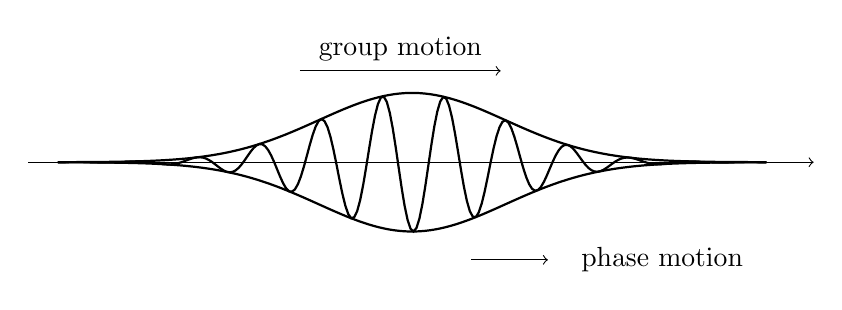
\begin{tikzpicture}[x=0.75cm,y=0.8cm]
\draw[->] (-0.5,0) -- (12.8,0);
\draw[thick] plot[domain=0:12,samples=140] (\x,{1.10*exp(-0.20*(\x-6)^2)});
\draw[thick] plot[domain=0:12,samples=140] (\x,{-1.10*exp(-0.20*(\x-6)^2)});
\draw[thick] plot[domain=0:12,samples=240] (\x,{1.10*exp(-0.20*(\x-6)^2)*sin(6*\x r)});
\draw[->] (4.1,1.45) -- (7.5,1.45);
\draw (5.8,1.8) node{group motion};
\draw[->] (7.0,-1.55) -- (8.3,-1.55);
\draw (8.7,-1.55) node[right]{phase motion};
\end{tikzpicture}
\caption{Un paquete de ondas localizado cuya envolvente y fase interna, en general, se mueven a velocidades distintas.}
\end{figure}

La velocidad de fase es la velocidad de las crestas, los valles y las demás fases constantes de una componente monocromática. Para la relación de dispersión no relativista,
\begin{equation}
v_\phi=f\lambda=\frac{h}{2m\lambda}.
\end{equation}
Depende de la longitud de onda. Por tanto, las componentes con distintas longitudes de onda tienen distintas velocidades de fase, de modo que las crestas pueden desplazarse a través del paquete y este puede dispersarse. La velocidad de grupo es la velocidad del paquete en su conjunto y es la que se identifica con la partícula.

Hay un caso particular sencillo. Si todas las componentes de longitud de onda se mueven con la misma velocidad, las velocidades de fase y de grupo coinciden. La luz en el vacío tiene esta propiedad: todas las longitudes de onda se propagan a \(c\). La relación para partículas lentas no la cumple; su valor de \(f\lambda\) cambia con \(\lambda\).

La ecuación
\begin{equation}
f=\frac{h}{2m\lambda^2}
\end{equation}
es la ecuación libre de Schr\"odinger escrita de una forma algo disfrazada. La frecuencia especifica la dependencia temporal de una onda plana, la longitud de onda especifica su dependencia espacial y la ecuación de Schr\"odinger relaciona ambas. A la inversa, al sustituir una onda de frecuencia y longitud de onda definidas en la ecuación libre de Schr\"odinger, se obtiene de nuevo esta relación de dispersión.

\begin{classroomqa}
\lecturetimestamp{00:47:02}
\audiencequestion{¿Puede la velocidad de fase superar la velocidad de la luz?}
\lecturerresponse{Sí. La velocidad de fase no transporta información. La información y el paquete localizado se propagan con la velocidad de grupo, así que una velocidad de fase superlumínica no permite transmitir señales más rápido que la luz.}
\end{classroomqa}

\section{Espacio finito y momento discreto}

Nos interesan finalmente las ondas en un espacio infinito, pero es más seguro empezar con un sistema finito. Un ordenador no puede almacenar ni manipular directamente el infinito. Primero se formulan las ecuaciones para un sistema finito y solo después se toma el límite en el que su tamaño se hace arbitrariamente grande. Este método resulta útil en toda la mecánica cuántica, la teoría cuántica de campos y la física de partículas.

No se pierde nada esencial al empezar en una dimensión espacial. La onda podría estar en una cuerda de violín, en una cuerda que se hace vibrar o en un mundo abstracto unidimensional. El sistema finito más evidente es un segmento de longitud \(L\) con extremos reflectantes. La onda llega a un extremo, se refleja y vuelve. Esta es una condición de contorno reflectante perfectamente válida, pero tiene un inconveniente: el momento no se conserva dentro del sistema de ondas. Una onda que se desplaza hacia la derecha lleva momento hacia la derecha; después de reflejarse, lo lleva hacia la izquierda. El contorno ha proporcionado el impulso y absorbido la diferencia.

La inversión del momento en un extremo reflectante puede representarse esquemáticamente.\footnote{El esquema sigue el argumento sobre los contornos reflectantes en 00:49:24--00:51:08.}

\begin{figure}[t]
\centering
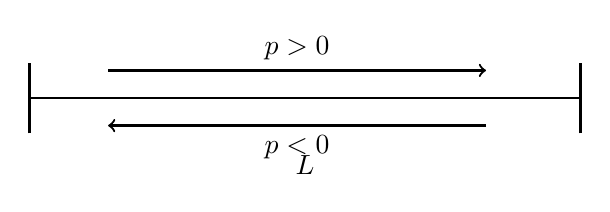
\begin{tikzpicture}[x=1cm,y=1cm]
\draw[thick] (0,0) -- (7,0);
\draw[very thick] (0,-0.45) -- (0,0.45);
\draw[very thick] (7,-0.45) -- (7,0.45);
\draw[->,thick] (1.0,0.35) -- (5.8,0.35) node[midway,above]{\(p>0\)};
\draw[->,thick] (5.8,-0.35) -- (1.0,-0.35) node[midway,below]{\(p<0\)};
\draw (3.5,-0.85) node{\(L\)};
\end{tikzpicture}
\caption{La reflexión en los extremos de un segmento finito invierte el momento de una onda viajera.}
\end{figure}

Hay otra forma de hacer finito el sistema y conservar el momento. Se identifican los dos extremos del segmento. El resultado puede dibujarse como un círculo, pero no hace falta que haya un círculo literal embebido en una segunda dimensión. La afirmación matemática es simplemente que la coordenada es periódica: tras recorrer una distancia total de \(L\), se vuelve al mismo punto.

\begin{figure}[t]
\centering
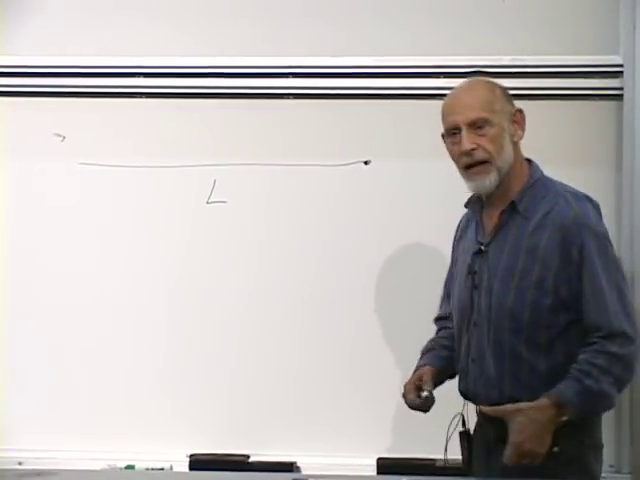
\includegraphics[width=0.72\textwidth]{lecture_02_figure_06.png}
\caption{Un recorrido unidimensional de longitud total \(L\) que sirve para introducir la identificación periódica.}
\lectureframe{00:51:21}
\end{figure}

El siguiente esquema muestra explícitamente la identificación de los extremos.\footnote{El esquema sigue el argumento sobre la identificación periódica en 00:51:09--00:52:37.}

\begin{figure}[t]
\centering
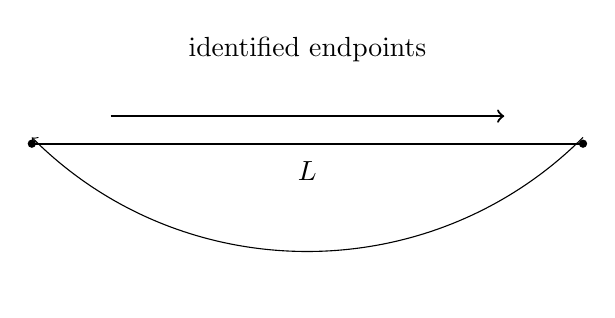
\begin{tikzpicture}[x=1cm,y=1cm]
\draw[thick] (0,0) -- (7,0);
\fill (0,0) circle (1.5pt);
\fill (7,0) circle (1.5pt);
\draw[->,thick] (1.0,0.35) -- (6.0,0.35);
\draw (3.5,-0.35) node{\(L\)};
\draw[->,bend left=45] (7,0.08) to (0,0.08);
\draw (3.5,1.2) node{identified endpoints};
\end{tikzpicture}
\caption{Espacio unidimensional periódico que se obtiene al identificar los extremos de un recorrido de longitud \(L\).}
\end{figure}

Una onda que se mueve hacia la derecha llega entonces al extremo representado, reaparece al comienzo y sigue moviéndose hacia la derecha. Una onda que se mueve hacia la izquierda sigue, de igual manera, moviéndose hacia la izquierda. No hay ningún extremo distinguido en el que la onda se refleje, así que el momento no se invierte. El espacio periódico hace que el volumen sea finito y conserva el momento, pero tiene una consecuencia importante: los momentos permitidos son discretos.

En la longitud total debe caber un número entero de longitudes de onda. Para un modo no constante,
\begin{equation}
\lambda_{|N|}=\frac{L}{|N|},
\qquad |N|=1,2,3,\ldots .
\end{equation}
Así, el módulo de la longitud de onda puede ser \(L\), \(L/2\), \(L/3\), y así sucesivamente. Una elección como \(L/\sqrt{2}\) no encaja: tras una vuelta, la onda regresaría con una fase incorrecta y no coincidiría con su valor inicial.

Usando \(p=h/\lambda\), el módulo del momento del modo no constante \(|N|\) es
\begin{equation}
|p_N|=\frac{|N|h}{L}.
\end{equation}
Para incluir sin ambigüedad ambas direcciones y el modo constante, conviene que la etiqueta del modo tenga signo:
\begin{equation}
p_N=\frac{Nh}{L},
\qquad N=0,\pm1,\pm2,\ldots .
\end{equation}
Los valores positivos y negativos de \(N\) describen direcciones de propagación opuestas. El modo \(N=0\) es constante y tiene momento nulo; no tiene una longitud de onda finita que pueda sustituirse en \(h/\lambda\). Por tanto, el espaciado básico entre valores del momento es \(h/L\).

Para un \(L\) macroscópico, tanto \(h\) como \(1/L\) hacen que este espaciado sea extremadamente pequeño, de modo que los valores permitidos forman un conjunto muy denso y parecen casi continuos. Sin embargo, una cuenta restringida a un alambre circular tiene exactamente este espectro discreto.

\begin{classroomqa}
\lecturetimestamp{00:58:27}
\audiencequestion{¿La cantidad cuantizada es el momento total de la onda o el momento asociado a un período?}
\lecturerresponse{La afirmación se refiere al momento de cada cuanto. Cada cuanto tiene uno de los momentos discretos permitidos. Por consiguiente, el momento total de cualquier conjunto de cuantos también es un múltiplo entero de la unidad básica \(h/L\).}
\end{classroomqa}

\begin{classroomqa}
\lecturetimestamp{00:59:22}
\audiencequestion{¿Por qué la onda debe regresar al mismo valor después de una vuelta?}
\lecturerresponse{Los extremos identificados son el mismo punto físico, así que un campo observable debe tener el mismo valor en ambos. Una discrepancia exigiría un salto repentino del campo en ese punto. Una discontinuidad así tiene un coste energético y de momento; las configuraciones de campo admisibles son continuas y periódicas.}
\end{classroomqa}

\begin{classroomqa}
\lecturetimestamp{01:00:09}
\audiencequestion{¿Qué ocurre si la onda está localizada en un paquete?}
\lecturerresponse{Un paquete es una suma de Fourier de ondas planas o, de forma equivalente, de senos y cosenos. En un espacio periódico, esa suma solo puede contener los modos de momento discretos permitidos. Por tanto, la cuantización se refiere a las componentes de Fourier de cualquier paquete admisible.}
\end{classroomqa}

\begin{classroomqa}
\lecturetimestamp{01:01:01}
\audiencequestion{¿Hay algún problema si la longitud periódica \(L\) se vuelve extremadamente pequeña?}
\lecturerresponse{Al disminuir \(L\), el momento básico \(h/L\) se vuelve muy grande. En longitudes microscópicas ordinarias no se desprende de ello ninguna inconsistencia inmediata, pero se espera que intentar llevar esta construcción hasta la escala de la longitud de Planck requiera nueva física.}
\end{classroomqa}

Tomemos ahora literalmente la imagen circular: una cuenta se mueve sobre un alambre circular de radio \(r\), cuya circunferencia es \(L=2\pi r\). Sus momentos tangenciales permitidos son
\begin{equation}
p_N=\frac{Nh}{2\pi r}=\frac{N\hbar}{r}.
\end{equation}
Para una partícula no relativista en una órbita circular, el momento angular es \(mvr\). Como en ese régimen \(p=mv\), esto equivale a \(rp\). La expresión \(mvr\) no es válida en general relativistamente, porque entonces \(p\) no es simplemente \(mv\), pero el producto del momento por la distancia perpendicular sigue siendo la relación correcta. En forma vectorial,\footnote{En la clase, primero se usa \(L\) para el momento angular y luego se advierte que coincide con \(L\), usado para la longitud periódica, por lo que se cambia la notación. Aquí se usa \(J\) en todo momento; véase 01:03:40--01:05:21.}
\begin{equation}
\vec J=\vec r\times\vec p,
\end{equation}
y, para el movimiento circular tangencial, su módulo es \(J=rp\). Por tanto,
\begin{equation}
J_N=rp_N=N\hbar.
\end{equation}
El espaciado del momento lineal depende del tamaño del círculo, mientras que la unidad del momento angular siempre es \(\hbar\). Hay excepciones a la regla de los enteros cuando intervienen fermiones; se posponen para más adelante.

El siguiente paso es establecer con mayor precisión el vínculo entre los campos, las partículas y los cuantos. Para ello hay que volver brevemente a la mecánica cuántica de los operadores y del oscilador armónico.

\section{Modos de onda y operadores cuánticos}

La mecánica cuántica que sigue es necesariamente abstracta y se presenta a modo de repaso. El oscilador armónico es el sistema esencial porque una onda es una oscilación. En un punto fijo, un campo eléctrico, un campo magnético o cualquier otra amplitud ondulatoria varía periódicamente en el tiempo; decir que una componente tiene una frecuencia ya significa que oscila.

Una onda general no tiene por qué tener una sola longitud de onda. Se pueden mezclar luces de varios colores y, a la inversa, un prisma puede separar la luz mezclada en sus colores componentes, como en la descomposición de la luz blanca de Newton. Cada componente tiene su propia longitud de onda, frecuencia, amplitud, energía y momento. Así, la onda mezclada puede descomponerse en cuantos de distintas energías y momentos. Cada longitud de onda determina una frecuencia, y cada componente de frecuencia definida se comporta como un oscilador. Por eso, el oscilador armónico, y no un sistema cuántico arbitrario, es el elemento básico natural de un campo.

Los observables cuánticos se representan mediante operadores. Los operadores se pueden sumar y multiplicar, pero, a diferencia de los números ordinarios, sus productos no tienen por qué ser independientes del orden. Sean \(A\) y \(B\) dos propiedades de un sistema, cada una de las cuales podría medirse por separado. Por ejemplo, \(A\) podría representar un campo eléctrico y \(B\), un campo magnético. Si los valores medidos son los números ordinarios \(a\) y \(b\), entonces
\begin{equation}
ab=ba.
\end{equation}
Su producto numérico no puede depender del orden de la multiplicación. En mecánica cuántica, en cambio, los operadores correspondientes pueden satisfacer \(AB-BA\neq0\).

A primera vista, esto parece absurdo. Si al medir el campo eléctrico se obtiene un número y al medir el campo magnético se obtiene otro, el producto de esos dos números debe dar el mismo resultado en cualquier orden. La solución es que, cuando los productos de los operadores dependen del orden, las dos cantidades no se pueden medir simultáneamente. El experimento que mide una interfiere con la medición de la otra. No hay contradicción, porque no se pueden obtener ambos valores numéricos a la vez.

Cuando dos cantidades se pueden medir simultáneamente, sus valores medidos son números ordinarios y conmutan. Por tanto, la prueba de si se pueden medir simultáneamente es el conmutador
\begin{equation}
[A,B]=AB-BA.
\end{equation}
Un conmutador nulo significa que los observables son compatibles; uno distinto de cero significa que las mediciones correspondientes interfieren entre sí. Invertir el orden de los términos invierte el signo:
\begin{equation}
[B,A]=-[A,B].
\end{equation}

Para una partícula no relativista, las tres componentes de la posición conmutan entre sí, al igual que las tres componentes del momento:
\begin{align}
[x,y]&=[y,z]=[z,x]=0,\\
[p_x,p_y]&=[p_y,p_z]=[p_z,p_x]=0.
\end{align}
Se pueden especificar a la vez las tres coordenadas y también las tres componentes del momento. Las componentes correspondientes de la posición y el momento no conmutan:
\begin{equation}
[x,p_x]=[y,p_y]=[z,p_z]=i\hbar,
\end{equation}
mientras que los conmutadores entre componentes distintas, como \([x,p_y]\), se anulan. Medir una coordenada de posición perturba el momento conjugado de la partícula. Equivalentemente, el producto de las incertidumbres correspondientes de posición y momento está determinado por \(\hbar\).

\begin{classroomqa}
\lecturetimestamp{01:16:30}
\audiencequestion{Al pasar de \(x\) a \(y\), ¿debería cambiar \(i\) en el conmutador por \(j\)}
\lecturerresponse{No. El símbolo \(i\) representa siempre la unidad imaginaria, la raíz cuadrada de menos uno. No es una etiqueta de vector unitario cartesiano ni uno de los símbolos cuaterniónicos \(i,j,k\)}
\end{classroomqa}

\begin{classroomqa}
\lecturetimestamp{01:17:24}
\audiencequestion{¿Significa \(AB-BA\) medir primero \(A\) y después \(B\), y luego invertir el orden de las mediciones?}
\lecturerresponse{No. Los dos términos son productos de operadores o matrices en distintos órdenes algebraicos. No representan una secuencia literal de mediciones. La relación con las mediciones incompatibles es una consecuencia del álgebra de operadores, no la definición del producto.}
\end{classroomqa}

\begin{classroomqa}
\lecturetimestamp{01:18:32}
\audiencequestion{¿Se aplican directamente a un fotón estos conmutadores de posición--momento?}
\lecturerresponse{No directamente. Se aplican sin complicaciones a partículas no relativistas. La posición de un fotón es más difícil de definir, así que el enunciado análogo requiere más cuidado y no hace falta aquí.}
\end{classroomqa}

\section{El oscilador armónico cuántico}

Un peso sujeto a un resorte, una onda sonora y una onda luminosa son ejemplos de movimiento oscilatorio. Todo oscilador armónico ideal tiene una frecuencia. En el caso de un resorte, un período completo no es simplemente el tiempo que tarda el peso en volver a la misma posición; debe volver a esa posición moviéndose en la misma dirección. El número de períodos completos por segundo es \(f\), y \(\omega=2\pi f\).

Clásicamente, un oscilador ideal puede tener cualquier energía no negativa. Un empujón suave le da poca energía y uno más fuerte le da más. Un resorte real acabaría rompiéndose o fundiéndose, pero la idealización matemática tiene un continuo de energías positivas. El oscilador cuántico es distinto: sus energías permitidas forman una serie discreta y equiespaciada. Si se elige el origen de energía de modo que el nivel más bajo se llame cero,
\begin{equation}
E_n=n\hbar\omega,
\qquad n=0,1,2,\ldots .
\end{equation}
Los niveles equiespaciados se pueden representar así.\footnote{El esquema de niveles de energía sigue el análisis en la pizarra de 01:21:20--01:23:56.}

\begin{figure}[t]
\centering
\begin{tikzpicture}[x=1cm,y=0.9cm]
\draw[->] (0,0) -- (0,5.35);
\draw (0,5.5) node[above]{energy};
\foreach \y/\lab in {0.6/{0},1.6/{\hbar\omega},2.6/{2\hbar\omega},3.6/{3\hbar\omega},4.6/{n\hbar\omega}}
{
  \draw[thick] (0.2,\y) -- (2.2,\y);
  \draw (-0.25,\y) node[left]{\(\lab\)};
}
\draw[->,thick] (2.8,0.68) -- (2.8,1.52);
\draw (3.2,1.1) node[right]{\(a_+\)};
\draw[->,thick] (3.7,1.52) -- (3.7,0.68);
\draw (4.1,1.1) node[right]{\(a_-\)};
\end{tikzpicture}
\caption{Niveles equiespaciados del oscilador con la convención \(E_n=n\hbar\omega\)}
\end{figure}

La separación \(\hbar\omega\) es la misma energía que se asignó antes a un fotón de frecuencia angular \(\omega\). El valor \(2\hbar\omega\) podría ser la energía de un cuanto de un oscilador de frecuencia \(2\omega\), o la energía de dos cuantos en un oscilador de frecuencia \(\omega\). Aquí se necesita la segunda interpretación. Un solo oscilador de frecuencia fija puede contener cero, uno, dos, tres o más cuantos, sin que haya energías permitidas entre los escalones.

El entero \(n\) etiqueta el estado del oscilador, que se escribe como el ket \(|n\rangle\). El estado \(|0\rangle\) es el estado fundamental, \(|1\rangle\) tiene un cuanto de excitación, \(|2\rangle\) tiene dos, y así sucesivamente. El ket es simplemente la notación del estado sobre el que actúan los operadores.

Definamos un operador de ascenso \(a_+\) que sube un estado un nivel y un operador de descenso \(a_-\) que lo baja un nivel:
\begin{align}
a_+|n\rangle &= \sqrt{n+1}\,|n+1\rangle,\\
a_-|n\rangle &= \sqrt{n}\,|n-1\rangle.
\end{align}
Los factores numéricos de raíz cuadrada forman parte de las definiciones. Para el estado más bajo,
\begin{equation}
a_-|0\rangle=0,
\end{equation}
porque no hay ningún estado por debajo del estado fundamental.

Aquí es importante distinguir los números ordinarios de los operadores. La etiqueta \(n\) y los coeficientes como \(\sqrt n\) son números ordinarios; conmutan con todo. Los símbolos \(a_+\) y \(a_-\) son operadores, y debe preservarse su orden.

Primero se baja \(|n\rangle\) y luego se vuelve a subir. El paso de descenso da
\begin{equation}
a_-|n\rangle=\sqrt n\,|n-1\rangle.
\end{equation}
Al actuar sobre el estado resultante, \(a_+\) aporta otro factor \(\sqrt n\), porque al subir \(|n-1\rangle\) se vuelve a \(|n\rangle\):
\begin{align}
a_+a_-|n\rangle
&=a_+\bigl(\sqrt n\,|n-1\rangle\bigr)\\
&=\sqrt n\,\sqrt n\,|n\rangle\\
&=n|n\rangle.
\end{align}
Así, \(a_+a_-\) lee el número de nivel. Por ejemplo, supongamos que se sabe que \(|\chi\rangle\) es un autoestado del número, pero se desconoce su etiqueta de nivel. Si
\begin{equation}
a_+a_-|\chi\rangle=q|\chi\rangle,
\end{equation}
entonces el coeficiente numérico ordinario \(q\) es el número de cuantos de ese estado. Por tanto, el producto es el operador número,
\begin{equation}
\hat n=a_+a_-,
\end{equation}
y, con la convención de energía elegida, el Hamiltoniano es
\begin{equation}
H=\hbar\omega\,a_+a_-.
\end{equation}
En efecto, al actuar sobre cualquier nivel da \(H|n\rangle=n\hbar\omega|n\rangle\).

Ahora invirtamos el orden. Primero, el ascenso da \(\sqrt{n+1}|n+1\rangle\). Luego, el descenso vuelve a \(|n\rangle\) y aporta un segundo factor \(\sqrt{n+1}\):
\begin{align}
a_-a_+|n\rangle
&=a_-\bigl(\sqrt{n+1}\,|n+1\rangle\bigr)\\
&=\sqrt{n+1}\,\sqrt{n+1}\,|n\rangle\\
&=(n+1)|n\rangle.
\end{align}
Los dos órdenes difieren en una unidad en todos los estados, así que
\begin{equation}
[a_-,a_+]=a_-a_+-a_+a_-=1.
\end{equation}

El oscilador también tiene amplitud y fase. La fase especifica en qué punto de su ciclo se encuentra; en concreto, puede fijarse mediante el instante en que el oscilador pasa por el origen en una dirección determinada. Retrasar ese paso cambia la fase sin cambiar la frecuencia. Los operadores escalera combinan las variables cuánticas asociadas a la amplitud y la fase. Su álgebra es intrínsecamente cuántica, pero su acción es sencilla: \(a_+\) añade un cuanto de energía del oscilador y \(a_-\) quita uno. En un modo electromagnético, esos cuantos son fotones, por lo que los dos operadores se llaman operadores de creación y aniquilación.

\begin{classroomqa}
\lecturetimestamp{01:37:34}
\audiencequestion{¿Corresponden los operadores de ascenso y descenso a una medición física?}
\lecturerresponse{El número de fotones es medible. Los operadores \(a_+\) y \(a_-\) no son observables medibles por separado, por otras razones técnicas. Su conmutador muestra que no conmutan entre sí, pero ese hecho por sí solo no constituye el argumento de que cada uno sea inobservable por separado.}
\end{classroomqa}

Un conjunto de resortes con distintas frecuencias naturales da lugar a muchos osciladores independientes. Lo mismo ocurre con los modos electromagnéticos de una cavidad: se puede excitar una longitud de onda sin que las demás tengan que presentar la misma excitación. En mecánica cuántica, los operadores de creación y aniquilación añaden y quitan cuantos de frecuencia fija en cada oscilador independiente. Este lenguaje es fundamental porque las partículas se identificarán precisamente con esos cuantos.

\section{Un campo como conjunto de osciladores}

Volvamos al espacio unidimensional periódico de longitud total \(L\). Sus modos no constantes tienen magnitudes de longitud de onda
\begin{equation}
\lambda_N=\frac{L}{N},
\qquad N=1,2,3,\ldots ,
\end{equation}
y las correspondientes frecuencias angulares no negativas \(\omega_N\). Para compararlas con el espectro de momentos anterior, resulta útil volver a etiquetar su entero con signo mediante \(M\):
\begin{equation}
p_M=\frac{Mh}{L},
\qquad M=0,\pm1,\pm2,\ldots .
\end{equation}
El signo de \(M\) indica la dirección de propagación.
\editorialnote{En 01:42:08--01:42:24 se corrige el índice del modo de frecuencia: pasa de un intervalo con signo a uno que comienza en cero y aumenta. Aquí el símbolo \(M\) se usa únicamente para mantener separada la notación de momento con signo de la etiqueta no negativa del modo de frecuencia \(N\); no introduce ocupaciones independientes para \(+M\) y \(-M\). La lista de osciladores no constantes comienza en \(N=1\).}

Cada frecuencia permitida se comporta como un oscilador armónico. Se puede añadir energía primero a una frecuencia y luego a otra, de manera independiente. El ejemplo detallado del primer campo cuántico se deja para la próxima lección, pero la notación de los estados ya está clara. Ordenando los modos no constantes desde la longitud de onda más larga, escribimos
\begin{equation}
|n_1,n_2,n_3,\ldots\rangle,
\end{equation}
donde \(n_N=0,1,2,\ldots\) es el número de cuantos en el oscilador de frecuencia \(\omega_N\). La primera entrada indica cuántos cuantos ocupan el modo de mayor longitud de onda; la segunda indica cuántos ocupan el siguiente modo, y así sucesivamente sin fin.

Los armónicos de una cuerda concretan esta construcción. Se muestra esquemáticamente la progresión desde el modo fundamental hasta los dos armónicos siguientes.\footnote{El esquema sigue la explicación de los armónicos de una cuerda en 01:45:20--01:47:46.}

\begin{figure}[t]
\centering
\resizebox{\linewidth}{!}{%
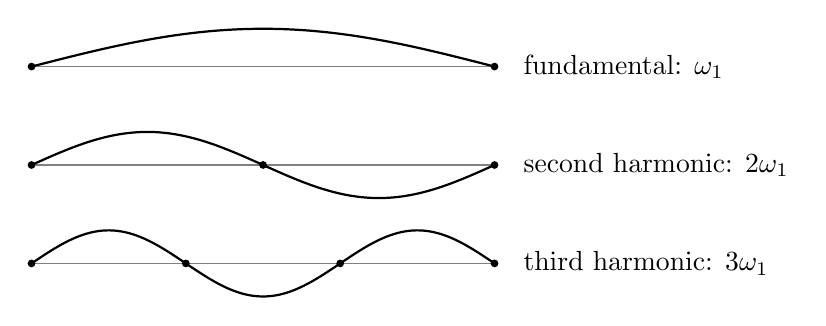
\begin{tikzpicture}[x=0.98cm,y=1cm]
\draw[gray] (0,2.5) -- (6,2.5);
\draw[thick] plot[domain=0:6,samples=120] (\x,{2.5+0.48*sin(30*\x)});
\fill (0,2.5) circle (1.4pt);
\fill (6,2.5) circle (1.4pt);
\node[right] at (6.25,2.5) {fundamental: \(\omega_1\)};

\draw[gray] (0,1.25) -- (6,1.25);
\draw[thick] plot[domain=0:6,samples=120] (\x,{1.25+0.42*sin(60*\x)});
\fill (0,1.25) circle (1.4pt);
\fill (3,1.25) circle (1.4pt);
\fill (6,1.25) circle (1.4pt);
\node[right] at (6.25,1.25) {second harmonic: \(2\omega_1\)};

\draw[gray] (0,0) -- (6,0);
\draw[thick] plot[domain=0:6,samples=120] (\x,{0.42*sin(90*\x)});
\fill (0,0) circle (1.4pt);
\fill (2,0) circle (1.4pt);
\fill (4,0) circle (1.4pt);
\fill (6,0) circle (1.4pt);
\node[right] at (6.25,0) {third harmonic: \(3\omega_1\)};
\end{tikzpicture}%
}
\caption{El modo fundamental de la cuerda y sus armónicos segundo y tercero, con cero, uno y dos nodos interiores.}
\end{figure}

El modo fundamental se mueve como un arco amplio y no tiene nodos interiores. Es un oscilador, que puede contener \(n_1=0,1,2,\ldots\) cuantos; cada excitación cuesta \(\hbar\omega_1\). El segundo armónico tiene un nodo interior y el doble de frecuencia. Si el modo fundamental suena como el do central, este modo suena como el do una octava más arriba. Tiene un número de ocupación independiente \(n_2\), y cada uno de sus cuantos cuesta \(\hbar\omega_2=2\hbar\omega_1\). El tercer armónico tiene dos nodos interiores y una frecuencia triple de la fundamental. Tiene su propio número de ocupación independiente \(n_3\), que también puede ser cualquier entero no negativo.

Modo por modo, con la convención de energía usada arriba, la energía es el número de ocupación multiplicado por la energía del cuanto. Al reunir esas contribuciones se obtiene
\begin{equation}
E=\sum_{N=1}^{\infty} n_N\hbar\omega_N.
\end{equation}
\editorialnote{Esta suma mostrada reúne algebraicamente las energías de los modos, enunciadas por separado en 01:44:02--01:47:46.}

Hay que repetir las mismas matemáticas del oscilador armónico para cada modo del campo, con un operador de creación y uno de aniquilación por cada oscilador independiente. En esta primera imagen elemental, un campo cuántico es el conjunto completo de esos osciladores y su álgebra de creación--aniquilación.

Este lenguaje se adapta a la dispersión de partículas. En un experimento entran cuantos con energía y momento definidos, y salen cuantos con otras energías y momentos. Los operadores de aniquilación eliminan las partículas iniciales; los operadores de creación de los modos apropiados insertan las partículas salientes en el estado final.

\begin{classroomqa}
\lecturetimestamp{01:49:38}
\audiencequestion{¿Se usa el mismo entero para etiquetar el modo del oscilador y contar el número de cuantos que contiene?}
\lecturerresponse{Hay dos enteros distintos. La etiqueta del modo \(N\) identifica el patrón espacial; en el ejemplo de la cuerda, su número de nodos determina la frecuencia \(\omega_N\). El número de ocupación \(n_N\) indica cuántos cuantos tienen esa frecuencia.}
\end{classroomqa}